\documentclass[1p]{elsarticle_modified}
%\bibliographystyle{elsarticle-num}

%\usepackage[colorlinks]{hyperref}
%\usepackage{abbrmath_seonhwa} %\Abb, \Ascr, \Acal ,\Abf, \Afrak
\usepackage{amsfonts}
\usepackage{amssymb}
\usepackage{amsmath}
\usepackage{amsthm}
\usepackage{scalefnt}
\usepackage{amsbsy}
\usepackage{kotex}
\usepackage{caption}
\usepackage{subfig}
\usepackage{color}
\usepackage{graphicx}
\usepackage{xcolor} %% white, black, red, green, blue, cyan, magenta, yellow
\usepackage{float}
\usepackage{setspace}
\usepackage{hyperref}

\usepackage{tikz}
\usetikzlibrary{arrows}

\usepackage{multirow}
\usepackage{array} % fixed length table
\usepackage{hhline}

%%%%%%%%%%%%%%%%%%%%%
\makeatletter
\renewcommand*\env@matrix[1][\arraystretch]{%
	\edef\arraystretch{#1}%
	\hskip -\arraycolsep
	\let\@ifnextchar\new@ifnextchar
	\array{*\c@MaxMatrixCols c}}
\makeatother %https://tex.stackexchange.com/questions/14071/how-can-i-increase-the-line-spacing-in-a-matrix
%%%%%%%%%%%%%%%

\usepackage[normalem]{ulem}

\newcommand{\msout}[1]{\ifmmode\text{\sout{\ensuremath{#1}}}\else\sout{#1}\fi}
%SOURCE: \msout is \stkout macro in https://tex.stackexchange.com/questions/20609/strikeout-in-math-mode

\newcommand{\cancel}[1]{
	\ifmmode
	{\color{red}\msout{#1}}
	\else
	{\color{red}\sout{#1}}
	\fi
}

\newcommand{\add}[1]{
	{\color{blue}\uwave{#1}}
}

\newcommand{\replace}[2]{
	\ifmmode
	{\color{red}\msout{#1}}{\color{blue}\uwave{#2}}
	\else
	{\color{red}\sout{#1}}{\color{blue}\uwave{#2}}
	\fi
}

\newcommand{\Sol}{\mathcal{S}} %segment
\newcommand{\D}{D} %diagram
\newcommand{\A}{\mathcal{A}} %arc


%%%%%%%%%%%%%%%%%%%%%%%%%%%%%5 test

\def\sl{\operatorname{\textup{SL}}(2,\Cbb)}
\def\psl{\operatorname{\textup{PSL}}(2,\Cbb)}
\def\quan{\mkern 1mu \triangleright \mkern 1mu}

\theoremstyle{definition}
\newtheorem{thm}{Theorem}[section]
\newtheorem{prop}[thm]{Proposition}
\newtheorem{lem}[thm]{Lemma}
\newtheorem{ques}[thm]{Question}
\newtheorem{cor}[thm]{Corollary}
\newtheorem{defn}[thm]{Definition}
\newtheorem{exam}[thm]{Example}
\newtheorem{rmk}[thm]{Remark}
\newtheorem{alg}[thm]{Algorithm}

\newcommand{\I}{\sqrt{-1}}
\begin{document}

%\begin{frontmatter}
%
%\title{Boundary parabolic representations of knots up to 8 crossings}
%
%%% Group authors per affiliation:
%\author{Yunhi Cho} 
%\address{Department of Mathematics, University of Seoul, Seoul, Korea}
%\ead{yhcho@uos.ac.kr}
%
%
%\author{Seonhwa Kim} %\fnref{s_kim}}
%\address{Center for Geometry and Physics, Institute for Basic Science, Pohang, 37673, Korea}
%\ead{ryeona17@ibs.re.kr}
%
%\author{Hyuk Kim}
%\address{Department of Mathematical Sciences, Seoul National University, Seoul 08826, Korea}
%\ead{hyukkim@snu.ac.kr}
%
%\author{Seokbeom Yoon}
%\address{Department of Mathematical Sciences, Seoul National University, Seoul, 08826,  Korea}
%\ead{sbyoon15@snu.ac.kr}
%
%\begin{abstract}
%We find all boundary parabolic representation of knots up to 8 crossings.
%
%\end{abstract}
%\begin{keyword}
%    \MSC[2010] 57M25 
%\end{keyword}
%
%\end{frontmatter}

%\linenumbers
%\tableofcontents
%
\newcommand\colored[1]{\textcolor{white}{\rule[-0.35ex]{0.8em}{1.4ex}}\kern-0.8em\color{red} #1}%
%\newcommand\colored[1]{\textcolor{white}{ #1}\kern-2.17ex	\textcolor{white}{ #1}\kern-1.81ex	\textcolor{white}{ #1}\kern-2.15ex\color{red}#1	}

{\Large $\underline{12n_{0081}~(K12n_{0081})}$}

\setlength{\tabcolsep}{10pt}
\renewcommand{\arraystretch}{1.6}
\vspace{1cm}\begin{tabular}{m{100pt}>{\centering\arraybackslash}m{274pt}}
\multirow{5}{120pt}{
	\centering
	\includegraphics[width=112pt]{../../../GIT/diagram.site/Diagrams/png/2170_12n_0081.png}\\
\ \ \ A knot diagram\footnotemark}&
\allowdisplaybreaks
\textbf{Linearized knot diagam} \\
\cline{2-2}
 &
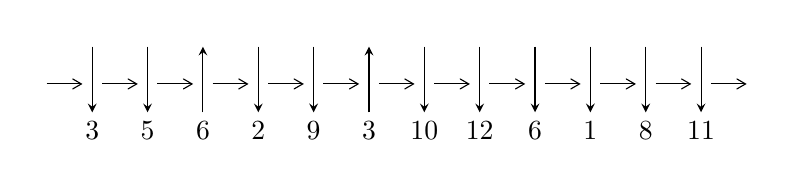
\begin{tikzpicture}[x=20pt, y=17pt]
	% nodes
	\node (C0) at (0, 0) {};
	\node (C1) at (1, 0) {};
	\node (C1U) at (1, +1) {};
	\node (C1D) at (1, -1) {3};

	\node (C2) at (2, 0) {};
	\node (C2U) at (2, +1) {};
	\node (C2D) at (2, -1) {5};

	\node (C3) at (3, 0) {};
	\node (C3U) at (3, +1) {};
	\node (C3D) at (3, -1) {6};

	\node (C4) at (4, 0) {};
	\node (C4U) at (4, +1) {};
	\node (C4D) at (4, -1) {2};

	\node (C5) at (5, 0) {};
	\node (C5U) at (5, +1) {};
	\node (C5D) at (5, -1) {9};

	\node (C6) at (6, 0) {};
	\node (C6U) at (6, +1) {};
	\node (C6D) at (6, -1) {3};

	\node (C7) at (7, 0) {};
	\node (C7U) at (7, +1) {};
	\node (C7D) at (7, -1) {10};

	\node (C8) at (8, 0) {};
	\node (C8U) at (8, +1) {};
	\node (C8D) at (8, -1) {12};

	\node (C9) at (9, 0) {};
	\node (C9U) at (9, +1) {};
	\node (C9D) at (9, -1) {6};

	\node (C10) at (10, 0) {};
	\node (C10U) at (10, +1) {};
	\node (C10D) at (10, -1) {1};

	\node (C11) at (11, 0) {};
	\node (C11U) at (11, +1) {};
	\node (C11D) at (11, -1) {8};

	\node (C12) at (12, 0) {};
	\node (C12U) at (12, +1) {};
	\node (C12D) at (12, -1) {11};
	\node (C13) at (13, 0) {};

	% arrows
	\draw[->,>={angle 60}]
	(C0) edge (C1) (C1) edge (C2) (C2) edge (C3) (C3) edge (C4) (C4) edge (C5) (C5) edge (C6) (C6) edge (C7) (C7) edge (C8) (C8) edge (C9) (C9) edge (C10) (C10) edge (C11) (C11) edge (C12) (C12) edge (C13) ;	\draw[->,>=stealth]
	(C1U) edge (C1D) (C2U) edge (C2D) (C3D) edge (C3U) (C4U) edge (C4D) (C5U) edge (C5D) (C6D) edge (C6U) (C7U) edge (C7D) (C8U) edge (C8D) (C9U) edge (C9D) (C10U) edge (C10D) (C11U) edge (C11D) (C12U) edge (C12D) ;
	\end{tikzpicture} \\
\hhline{~~} \\& 
\textbf{Solving Sequence} \\ \cline{2-2} 
 &
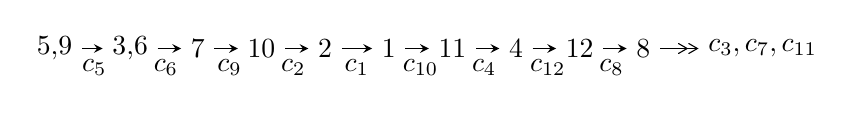
\begin{tikzpicture}[x=23pt, y=7pt]
	% node
	\node (A0) at (-1/8, 0) {5,9};
	\node (A1) at (17/16, 0) {3,6};
	\node (A2) at (17/8, 0) {7};
	\node (A3) at (25/8, 0) {10};
	\node (A4) at (33/8, 0) {2};
	\node (A5) at (41/8, 0) {1};
	\node (A6) at (49/8, 0) {11};
	\node (A7) at (57/8, 0) {4};
	\node (A8) at (65/8, 0) {12};
	\node (A9) at (73/8, 0) {8};
	\node (C1) at (1/2, -1) {$c_{5}$};
	\node (C2) at (13/8, -1) {$c_{6}$};
	\node (C3) at (21/8, -1) {$c_{9}$};
	\node (C4) at (29/8, -1) {$c_{2}$};
	\node (C5) at (37/8, -1) {$c_{1}$};
	\node (C6) at (45/8, -1) {$c_{10}$};
	\node (C7) at (53/8, -1) {$c_{4}$};
	\node (C8) at (61/8, -1) {$c_{12}$};
	\node (C9) at (69/8, -1) {$c_{8}$};
	\node (A10) at (11, 0) {$c_{3},c_{7},c_{11}$};

	% edge
	\draw[->,>=stealth]	
	(A0) edge (A1) (A1) edge (A2) (A2) edge (A3) (A3) edge (A4) (A4) edge (A5) (A5) edge (A6) (A6) edge (A7) (A7) edge (A8) (A8) edge (A9) ;
	\draw[->>,>={angle 60}]	
	(A9) edge (A10);
\end{tikzpicture} \\ 

\end{tabular} \\

\footnotetext{
The image of knot diagram is generated by the software ``\textbf{Draw programme}" developed by Andrew Bartholomew(\url{http://www.layer8.co.uk/maths/draw/index.htm\#Running-draw}), where we modified some parts for our purpose(\url{https://github.com/CATsTAILs/LinksPainter}).
}\phantom \\ \newline 
\centering \textbf{Ideals for irreducible components\footnotemark of $X_{\text{par}}$} 
 
\begin{align*}
I^u_{1}&=\langle 
5.53432\times10^{85} u^{57}-8.84907\times10^{85} u^{56}+\cdots+1.15940\times10^{86} b-1.39649\times10^{85},\\
\phantom{I^u_{1}}&\phantom{= \langle  }2.61940\times10^{85} u^{57}-5.40341\times10^{85} u^{56}+\cdots+2.31879\times10^{85} a-2.38511\times10^{85},\;u^{58}-2 u^{57}+\cdots- u+1\rangle \\
I^u_{2}&=\langle 
b+1,\;2 u^7+3 u^6-5 u^5-7 u^4+4 u^3+3 u^2+a+4,\;u^8+u^7-3 u^6-2 u^5+3 u^4+2 u-1\rangle \\
\\
\end{align*}
\raggedright * 2 irreducible components of $\dim_{\mathbb{C}}=0$, with total 66 representations.\\
\footnotetext{All coefficients of polynomials are rational numbers. But the coefficients are sometimes approximated in decimal forms when there is not enough margin.}
\newpage
\renewcommand{\arraystretch}{1}
\centering \section*{I. $I^u_{1}= \langle 5.53\times10^{85} u^{57}-8.85\times10^{85} u^{56}+\cdots+1.16\times10^{86} b-1.40\times10^{85},\;2.62\times10^{85} u^{57}-5.40\times10^{85} u^{56}+\cdots+2.32\times10^{85} a-2.39\times10^{85},\;u^{58}-2 u^{57}+\cdots- u+1 \rangle$}
\flushleft \textbf{(i) Arc colorings}\\
\begin{tabular}{m{7pt} m{180pt} m{7pt} m{180pt} }
\flushright $a_{5}=$&$\begin{pmatrix}1\\0\end{pmatrix}$ \\
\flushright $a_{9}=$&$\begin{pmatrix}0\\u\end{pmatrix}$ \\
\flushright $a_{3}=$&$\begin{pmatrix}-1.12964 u^{57}+2.33027 u^{56}+\cdots-0.0189625 u+1.02860\\-0.477346 u^{57}+0.763249 u^{56}+\cdots+1.48654 u+0.120450\end{pmatrix}$ \\
\flushright $a_{6}=$&$\begin{pmatrix}1\\u^2\end{pmatrix}$ \\
\flushright $a_{7}=$&$\begin{pmatrix}-0.742987 u^{57}+1.16928 u^{56}+\cdots+2.16233 u+0.683441\\-0.147869 u^{57}+0.246417 u^{56}+\cdots+0.573664 u+0.388653\end{pmatrix}$ \\
\flushright $a_{10}=$&$\begin{pmatrix}- u\\- u^3+u\end{pmatrix}$ \\
\flushright $a_{2}=$&$\begin{pmatrix}-1.60699 u^{57}+3.09352 u^{56}+\cdots+1.46757 u+1.14905\\-0.477346 u^{57}+0.763249 u^{56}+\cdots+1.48654 u+0.120450\end{pmatrix}$ \\
\flushright $a_{1}=$&$\begin{pmatrix}-0.768033 u^{57}+1.20204 u^{56}+\cdots+2.30970 u+0.755400\\0.0250459 u^{57}-0.0327586 u^{56}+\cdots-0.147371 u-0.0719590\end{pmatrix}$ \\
\flushright $a_{11}=$&$\begin{pmatrix}0.238196 u^{57}-0.406882 u^{56}+\cdots-2.56618 u-0.552552\\-0.0179618 u^{57}+0.0170715 u^{56}+\cdots+0.925015 u-0.0202253\end{pmatrix}$ \\
\flushright $a_{4}=$&$\begin{pmatrix}-1.20110 u^{57}+2.45056 u^{56}+\cdots+0.266941 u+1.22004\\-0.484972 u^{57}+0.772733 u^{56}+\cdots+1.53536 u+0.143087\end{pmatrix}$ \\
\flushright $a_{12}=$&$\begin{pmatrix}-0.842522 u^{57}+1.44178 u^{56}+\cdots+3.31034 u+1.38391\\0.240620 u^{57}-0.365565 u^{56}+\cdots-0.386959 u-0.465919\end{pmatrix}$ \\
\flushright $a_{8}=$&$\begin{pmatrix}-0.606276 u^{57}+0.938630 u^{56}+\cdots+1.72832 u+0.349414\\-0.275800 u^{57}+0.459793 u^{56}+\cdots+0.913732 u+0.679907\end{pmatrix}$\\&\end{tabular}
\flushleft \textbf{(ii) Obstruction class $= -1$}\\~\\
\flushleft \textbf{(iii) Cusp Shapes $= -1.20777 u^{57}+0.883719 u^{56}+\cdots-4.35534 u-9.32260$}\\~\\
\newpage\renewcommand{\arraystretch}{1}
\flushleft \textbf{(iv) u-Polynomials at the component}\newline \\
\begin{tabular}{m{50pt}|m{274pt}}
Crossings & \hspace{64pt}u-Polynomials at each crossing \\
\hline $$\begin{aligned}c_{1}\end{aligned}$$&$\begin{aligned}
&u^{58}+19 u^{57}+\cdots+1227 u+1
\end{aligned}$\\
\hline $$\begin{aligned}c_{2},c_{4}\end{aligned}$$&$\begin{aligned}
&u^{58}-9 u^{57}+\cdots-43 u+1
\end{aligned}$\\
\hline $$\begin{aligned}c_{3},c_{6}\end{aligned}$$&$\begin{aligned}
&u^{58}+7 u^{57}+\cdots+2688 u+256
\end{aligned}$\\
\hline $$\begin{aligned}c_{5},c_{9}\end{aligned}$$&$\begin{aligned}
&u^{58}+2 u^{57}+\cdots+u+1
\end{aligned}$\\
\hline $$\begin{aligned}c_{7}\end{aligned}$$&$\begin{aligned}
&u^{58}-2 u^{57}+\cdots+42759 u+8017
\end{aligned}$\\
\hline $$\begin{aligned}c_{8},c_{11}\end{aligned}$$&$\begin{aligned}
&u^{58}+2 u^{57}+\cdots+7 u+1
\end{aligned}$\\
\hline $$\begin{aligned}c_{10},c_{12}\end{aligned}$$&$\begin{aligned}
&u^{58}+18 u^{57}+\cdots+11 u+1
\end{aligned}$\\
\hline
\end{tabular}\\~\\
\newpage\renewcommand{\arraystretch}{1}
\flushleft \textbf{(v) Riley Polynomials at the component}\newline \\
\begin{tabular}{m{50pt}|m{274pt}}
Crossings & \hspace{64pt}Riley Polynomials at each crossing \\
\hline $$\begin{aligned}c_{1}\end{aligned}$$&$\begin{aligned}
&y^{58}+49 y^{57}+\cdots-1420135 y+1
\end{aligned}$\\
\hline $$\begin{aligned}c_{2},c_{4}\end{aligned}$$&$\begin{aligned}
&y^{58}-19 y^{57}+\cdots-1227 y+1
\end{aligned}$\\
\hline $$\begin{aligned}c_{3},c_{6}\end{aligned}$$&$\begin{aligned}
&y^{58}-51 y^{57}+\cdots-3719168 y+65536
\end{aligned}$\\
\hline $$\begin{aligned}c_{5},c_{9}\end{aligned}$$&$\begin{aligned}
&y^{58}-14 y^{57}+\cdots-11 y+1
\end{aligned}$\\
\hline $$\begin{aligned}c_{7}\end{aligned}$$&$\begin{aligned}
&y^{58}+22 y^{57}+\cdots+71584681 y+64272289
\end{aligned}$\\
\hline $$\begin{aligned}c_{8},c_{11}\end{aligned}$$&$\begin{aligned}
&y^{58}-18 y^{57}+\cdots-11 y+1
\end{aligned}$\\
\hline $$\begin{aligned}c_{10},c_{12}\end{aligned}$$&$\begin{aligned}
&y^{58}+46 y^{57}+\cdots-251 y+1
\end{aligned}$\\
\hline
\end{tabular}\\~\\
\newpage\flushleft \textbf{(vi) Complex Volumes and Cusp Shapes}
$$\begin{array}{c|c|c}  
\text{Solutions to }I^u_{1}& \I (\text{vol} + \sqrt{-1}CS) & \text{Cusp shape}\\
 \hline 
\begin{aligned}
u &= -0.757964 + 0.476676 I \\
a &= \phantom{-}0.211091 - 1.285110 I \\
b &= -0.733524 + 1.001690 I\end{aligned}
 & \phantom{-}1.39650 + 7.38606 I & -8.93309 - 9.73199 I \\ \hline\begin{aligned}
u &= -0.757964 - 0.476676 I \\
a &= \phantom{-}0.211091 + 1.285110 I \\
b &= -0.733524 - 1.001690 I\end{aligned}
 & \phantom{-}1.39650 - 7.38606 I & -8.93309 + 9.73199 I \\ \hline\begin{aligned}
u &= \phantom{-}0.733536 + 0.503634 I \\
a &= \phantom{-}0.207333 + 1.258410 I \\
b &= -0.622314 - 0.960850 I\end{aligned}
 & \phantom{-}1.93231 - 1.77262 I & -7.23531 + 4.32887 I \\ \hline\begin{aligned}
u &= \phantom{-}0.733536 - 0.503634 I \\
a &= \phantom{-}0.207333 - 1.258410 I \\
b &= -0.622314 + 0.960850 I\end{aligned}
 & \phantom{-}1.93231 + 1.77262 I & -7.23531 - 4.32887 I \\ \hline\begin{aligned}
u &= \phantom{-}0.150361 + 0.862598 I \\
a &= \phantom{-}0.283573 + 0.156210 I \\
b &= \phantom{-}0.296125 - 0.128802 I\end{aligned}
 & \phantom{-}1.86705 - 2.42873 I & -2.94093 + 3.38399 I \\ \hline\begin{aligned}
u &= \phantom{-}0.150361 - 0.862598 I \\
a &= \phantom{-}0.283573 - 0.156210 I \\
b &= \phantom{-}0.296125 + 0.128802 I\end{aligned}
 & \phantom{-}1.86705 + 2.42873 I & -2.94093 - 3.38399 I \\ \hline\begin{aligned}
u &= \phantom{-}0.729010 + 0.900450 I \\
a &= -0.278287 + 0.714115 I \\
b &= \phantom{-}0.512624 - 0.941655 I\end{aligned}
 & \phantom{-}1.79327 - 3.50993 I & -8.00000 + 0. I\phantom{ +0.000000I} \\ \hline\begin{aligned}
u &= \phantom{-}0.729010 - 0.900450 I \\
a &= -0.278287 - 0.714115 I \\
b &= \phantom{-}0.512624 + 0.941655 I\end{aligned}
 & \phantom{-}1.79327 + 3.50993 I & -8.00000 + 0. I\phantom{ +0.000000I} \\ \hline\begin{aligned}
u &= -0.707674 + 0.373154 I \\
a &= \phantom{-}0.190149 - 1.303650 I \\
b &= -0.946128 + 0.714336 I\end{aligned}
 & -3.61079 + 2.96792 I & -16.6955 - 7.6738 I \\ \hline\begin{aligned}
u &= -0.707674 - 0.373154 I \\
a &= \phantom{-}0.190149 + 1.303650 I \\
b &= -0.946128 - 0.714336 I\end{aligned}
 & -3.61079 - 2.96792 I & -16.6955 + 7.6738 I\\
 \hline 
 \end{array}$$\newpage$$\begin{array}{c|c|c}  
\text{Solutions to }I^u_{1}& \I (\text{vol} + \sqrt{-1}CS) & \text{Cusp shape}\\
 \hline 
\begin{aligned}
u &= \phantom{-}0.828609 + 0.884235 I \\
a &= -0.466481 + 0.852083 I \\
b &= \phantom{-}0.613518 - 1.215300 I\end{aligned}
 & \phantom{-}8.38484 - 8.22953 I & \phantom{-0.000000 } 0 \\ \hline\begin{aligned}
u &= \phantom{-}0.828609 - 0.884235 I \\
a &= -0.466481 - 0.852083 I \\
b &= \phantom{-}0.613518 + 1.215300 I\end{aligned}
 & \phantom{-}8.38484 + 8.22953 I & \phantom{-0.000000 } 0 \\ \hline\begin{aligned}
u &= -0.827954 + 0.902716 I \\
a &= -0.485901 - 0.807428 I \\
b &= \phantom{-}0.663928 + 1.180430 I\end{aligned}
 & \phantom{-}9.06399 + 2.20407 I & \phantom{-0.000000 } 0 \\ \hline\begin{aligned}
u &= -0.827954 - 0.902716 I \\
a &= -0.485901 + 0.807428 I \\
b &= \phantom{-}0.663928 - 1.180430 I\end{aligned}
 & \phantom{-}9.06399 - 2.20407 I & \phantom{-0.000000 } 0 \\ \hline\begin{aligned}
u &= \phantom{-}0.758547 + 0.131049 I \\
a &= -0.057075 + 0.644979 I \\
b &= -1.47907 - 0.32636 I\end{aligned}
 & -1.42978 - 4.33965 I & -13.8036 + 5.9098 I \\ \hline\begin{aligned}
u &= \phantom{-}0.758547 - 0.131049 I \\
a &= -0.057075 - 0.644979 I \\
b &= -1.47907 + 0.32636 I\end{aligned}
 & -1.42978 + 4.33965 I & -13.8036 - 5.9098 I \\ \hline\begin{aligned}
u &= -0.738708 + 0.184329 I \\
a &= -0.061286 - 0.888067 I \\
b &= -1.37022 + 0.42544 I\end{aligned}
 & -1.16921 - 0.90179 I & -13.10774 - 0.16863 I \\ \hline\begin{aligned}
u &= -0.738708 - 0.184329 I \\
a &= -0.061286 + 0.888067 I \\
b &= -1.37022 - 0.42544 I\end{aligned}
 & -1.16921 + 0.90179 I & -13.10774 + 0.16863 I \\ \hline\begin{aligned}
u &= -0.771402 + 0.979679 I \\
a &= -0.418138 - 0.593129 I \\
b &= \phantom{-}0.735262 + 0.914814 I\end{aligned}
 & \phantom{-}4.73839 + 0.20490 I & \phantom{-0.000000 } 0 \\ \hline\begin{aligned}
u &= -0.771402 - 0.979679 I \\
a &= -0.418138 + 0.593129 I \\
b &= \phantom{-}0.735262 - 0.914814 I\end{aligned}
 & \phantom{-}4.73839 - 0.20490 I & \phantom{-0.000000 } 0\\
 \hline 
 \end{array}$$\newpage$$\begin{array}{c|c|c}  
\text{Solutions to }I^u_{1}& \I (\text{vol} + \sqrt{-1}CS) & \text{Cusp shape}\\
 \hline 
\begin{aligned}
u &= \phantom{-}0.725261\phantom{ +0.000000I} \\
a &= -0.320581\phantom{ +0.000000I} \\
b &= -1.46548\phantom{ +0.000000I}\end{aligned}
 & -5.24110\phantom{ +0.000000I} & -20.4300\phantom{ +0.000000I} \\ \hline\begin{aligned}
u &= \phantom{-}1.010850 + 0.787058 I \\
a &= \phantom{-}0.82799 - 1.23601 I \\
b &= \phantom{-}0.817179 + 0.885590 I\end{aligned}
 & \phantom{-}7.78595 + 1.97085 I & \phantom{-0.000000 } 0 \\ \hline\begin{aligned}
u &= \phantom{-}1.010850 - 0.787058 I \\
a &= \phantom{-}0.82799 + 1.23601 I \\
b &= \phantom{-}0.817179 - 0.885590 I\end{aligned}
 & \phantom{-}7.78595 - 1.97085 I & \phantom{-0.000000 } 0 \\ \hline\begin{aligned}
u &= \phantom{-}0.747268 + 1.058050 I \\
a &= -0.395621 + 0.438566 I \\
b &= \phantom{-}0.813908 - 0.746877 I\end{aligned}
 & \phantom{-}1.08274 + 2.68379 I & \phantom{-0.000000 } 0 \\ \hline\begin{aligned}
u &= \phantom{-}0.747268 - 1.058050 I \\
a &= -0.395621 - 0.438566 I \\
b &= \phantom{-}0.813908 + 0.746877 I\end{aligned}
 & \phantom{-}1.08274 - 2.68379 I & \phantom{-0.000000 } 0 \\ \hline\begin{aligned}
u &= \phantom{-}0.562499 + 0.418736 I \\
a &= \phantom{-}0.47527 + 1.47284 I \\
b &= -0.667885 - 0.412194 I\end{aligned}
 & -0.84022 - 1.37563 I & -6.44015 + 4.83399 I \\ \hline\begin{aligned}
u &= \phantom{-}0.562499 - 0.418736 I \\
a &= \phantom{-}0.47527 - 1.47284 I \\
b &= -0.667885 + 0.412194 I\end{aligned}
 & -0.84022 + 1.37563 I & -6.44015 - 4.83399 I \\ \hline\begin{aligned}
u &= -1.021400 + 0.806453 I \\
a &= \phantom{-}0.76138 + 1.27349 I \\
b &= \phantom{-}0.872213 - 0.895148 I\end{aligned}
 & \phantom{-}8.43324 + 4.16970 I & \phantom{-0.000000 } 0 \\ \hline\begin{aligned}
u &= -1.021400 - 0.806453 I \\
a &= \phantom{-}0.76138 - 1.27349 I \\
b &= \phantom{-}0.872213 + 0.895148 I\end{aligned}
 & \phantom{-}8.43324 - 4.16970 I & \phantom{-0.000000 } 0 \\ \hline\begin{aligned}
u &= \phantom{-}0.464370 + 0.505657 I \\
a &= \phantom{-}2.19485 + 0.67921 I \\
b &= -0.485517 + 0.294137 I\end{aligned}
 & \phantom{-}2.55163 - 1.79957 I & -5.78089 + 4.77562 I\\
 \hline 
 \end{array}$$\newpage$$\begin{array}{c|c|c}  
\text{Solutions to }I^u_{1}& \I (\text{vol} + \sqrt{-1}CS) & \text{Cusp shape}\\
 \hline 
\begin{aligned}
u &= \phantom{-}0.464370 - 0.505657 I \\
a &= \phantom{-}2.19485 - 0.67921 I \\
b &= -0.485517 - 0.294137 I\end{aligned}
 & \phantom{-}2.55163 + 1.79957 I & -5.78089 - 4.77562 I \\ \hline\begin{aligned}
u &= \phantom{-}1.302260 + 0.215056 I \\
a &= \phantom{-}0.724570 - 0.182519 I \\
b &= \phantom{-}0.657572 + 0.133991 I\end{aligned}
 & -1.94270 - 1.43075 I & \phantom{-0.000000 } 0 \\ \hline\begin{aligned}
u &= \phantom{-}1.302260 - 0.215056 I \\
a &= \phantom{-}0.724570 + 0.182519 I \\
b &= \phantom{-}0.657572 - 0.133991 I\end{aligned}
 & -1.94270 + 1.43075 I & \phantom{-0.000000 } 0 \\ \hline\begin{aligned}
u &= -0.429870 + 0.520549 I \\
a &= \phantom{-}2.51794 - 0.86930 I \\
b &= -0.605155 - 0.307118 I\end{aligned}
 & \phantom{-}2.25105 - 3.87043 I & -6.73442 + 0.34200 I \\ \hline\begin{aligned}
u &= -0.429870 - 0.520549 I \\
a &= \phantom{-}2.51794 + 0.86930 I \\
b &= -0.605155 + 0.307118 I\end{aligned}
 & \phantom{-}2.25105 + 3.87043 I & -6.73442 - 0.34200 I \\ \hline\begin{aligned}
u &= -0.831079 + 1.050820 I \\
a &= -0.560219 - 0.451422 I \\
b &= \phantom{-}0.967229 + 0.864793 I\end{aligned}
 & \phantom{-}8.14146 - 2.33310 I & \phantom{-0.000000 } 0 \\ \hline\begin{aligned}
u &= -0.831079 - 1.050820 I \\
a &= -0.560219 + 0.451422 I \\
b &= \phantom{-}0.967229 - 0.864793 I\end{aligned}
 & \phantom{-}8.14146 + 2.33310 I & \phantom{-0.000000 } 0 \\ \hline\begin{aligned}
u &= \phantom{-}0.834599 + 1.071090 I \\
a &= -0.562906 + 0.405830 I \\
b &= \phantom{-}0.998315 - 0.821896 I\end{aligned}
 & \phantom{-}7.22076 + 8.31025 I & \phantom{-0.000000 } 0 \\ \hline\begin{aligned}
u &= \phantom{-}0.834599 - 1.071090 I \\
a &= -0.562906 - 0.405830 I \\
b &= \phantom{-}0.998315 + 0.821896 I\end{aligned}
 & \phantom{-}7.22076 - 8.31025 I & \phantom{-0.000000 } 0 \\ \hline\begin{aligned}
u &= \phantom{-}1.113430 + 0.804823 I \\
a &= \phantom{-}0.544448 - 1.077950 I \\
b &= \phantom{-}0.972357 + 0.706110 I\end{aligned}
 & \phantom{-}0.57880 - 2.87211 I & \phantom{-0.000000 } 0\\
 \hline 
 \end{array}$$\newpage$$\begin{array}{c|c|c}  
\text{Solutions to }I^u_{1}& \I (\text{vol} + \sqrt{-1}CS) & \text{Cusp shape}\\
 \hline 
\begin{aligned}
u &= \phantom{-}1.113430 - 0.804823 I \\
a &= \phantom{-}0.544448 + 1.077950 I \\
b &= \phantom{-}0.972357 - 0.706110 I\end{aligned}
 & \phantom{-}0.57880 + 2.87211 I & \phantom{-0.000000 } 0 \\ \hline\begin{aligned}
u &= -1.089310 + 0.851827 I \\
a &= \phantom{-}0.480537 + 1.230050 I \\
b &= \phantom{-}1.055730 - 0.794375 I\end{aligned}
 & \phantom{-}3.73913 + 6.53652 I & \phantom{-0.000000 } 0 \\ \hline\begin{aligned}
u &= -1.089310 - 0.851827 I \\
a &= \phantom{-}0.480537 - 1.230050 I \\
b &= \phantom{-}1.055730 + 0.794375 I\end{aligned}
 & \phantom{-}3.73913 - 6.53652 I & \phantom{-0.000000 } 0 \\ \hline\begin{aligned}
u &= -1.083120 + 0.904822 I \\
a &= \phantom{-}0.329084 + 1.363660 I \\
b &= \phantom{-}1.19685 - 0.84814 I\end{aligned}
 & \phantom{-}7.31786 + 9.44466 I & \phantom{-0.000000 } 0 \\ \hline\begin{aligned}
u &= -1.083120 - 0.904822 I \\
a &= \phantom{-}0.329084 - 1.363660 I \\
b &= \phantom{-}1.19685 + 0.84814 I\end{aligned}
 & \phantom{-}7.31786 - 9.44466 I & \phantom{-0.000000 } 0 \\ \hline\begin{aligned}
u &= \phantom{-}1.08928 + 0.91350 I \\
a &= \phantom{-}0.284481 - 1.359270 I \\
b &= \phantom{-}1.22723 + 0.83313 I\end{aligned}
 & \phantom{-}6.3813 - 15.5051 I & \phantom{-0.000000 } 0 \\ \hline\begin{aligned}
u &= \phantom{-}1.08928 - 0.91350 I \\
a &= \phantom{-}0.284481 + 1.359270 I \\
b &= \phantom{-}1.22723 - 0.83313 I\end{aligned}
 & \phantom{-}6.3813 + 15.5051 I & \phantom{-0.000000 } 0 \\ \hline\begin{aligned}
u &= \phantom{-}1.11634 + 0.88115 I \\
a &= \phantom{-}0.344161 - 1.208590 I \\
b &= \phantom{-}1.144810 + 0.743437 I\end{aligned}
 & -0.06948 - 9.72018 I & \phantom{-0.000000 } 0 \\ \hline\begin{aligned}
u &= \phantom{-}1.11634 - 0.88115 I \\
a &= \phantom{-}0.344161 + 1.208590 I \\
b &= \phantom{-}1.144810 - 0.743437 I\end{aligned}
 & -0.06948 + 9.72018 I & \phantom{-0.000000 } 0 \\ \hline\begin{aligned}
u &= -1.43228 + 0.28779 I \\
a &= \phantom{-}0.602581 + 0.217299 I \\
b &= \phantom{-}0.746089 - 0.144890 I\end{aligned}
 & -3.47621 + 6.76006 I & \phantom{-0.000000 } 0\\
 \hline 
 \end{array}$$\newpage$$\begin{array}{c|c|c}  
\text{Solutions to }I^u_{1}& \I (\text{vol} + \sqrt{-1}CS) & \text{Cusp shape}\\
 \hline 
\begin{aligned}
u &= -1.43228 - 0.28779 I \\
a &= \phantom{-}0.602581 - 0.217299 I \\
b &= \phantom{-}0.746089 + 0.144890 I\end{aligned}
 & -3.47621 - 6.76006 I & \phantom{-0.000000 } 0 \\ \hline\begin{aligned}
u &= -1.47635\phantom{ +0.000000I} \\
a &= \phantom{-}0.603436\phantom{ +0.000000I} \\
b &= \phantom{-}0.732744\phantom{ +0.000000I}\end{aligned}
 & -7.57251\phantom{ +0.000000I} & \phantom{-0.000000 } 0 \\ \hline\begin{aligned}
u &= -0.310564 + 0.379876 I \\
a &= \phantom{-}2.83067 - 3.52170 I \\
b &= -0.888180 - 0.051391 I\end{aligned}
 & -2.59810 - 0.31577 I & -24.5055 - 6.4182 I \\ \hline\begin{aligned}
u &= -0.310564 - 0.379876 I \\
a &= \phantom{-}2.83067 + 3.52170 I \\
b &= -0.888180 + 0.051391 I\end{aligned}
 & -2.59810 + 0.31577 I & -24.5055 + 6.4182 I \\ \hline\begin{aligned}
u &= -0.485729\phantom{ +0.000000I} \\
a &= -2.58176\phantom{ +0.000000I} \\
b &= -1.10599\phantom{ +0.000000I}\end{aligned}
 & -2.22309\phantom{ +0.000000I} & \phantom{-}1.58660\phantom{ +0.000000I} \\ \hline\begin{aligned}
u &= -0.030516 + 0.465574 I \\
a &= \phantom{-}7.05708 - 0.52655 I \\
b &= -1.088060 - 0.022657 I\end{aligned}
 & \phantom{-}0.94270 + 2.75058 I & \phantom{-}17.8156 - 8.6403 I \\ \hline\begin{aligned}
u &= -0.030516 - 0.465574 I \\
a &= \phantom{-}7.05708 + 0.52655 I \\
b &= -1.088060 + 0.022657 I\end{aligned}
 & \phantom{-}0.94270 - 2.75058 I & \phantom{-}17.8156 + 8.6403 I \\ \hline\begin{aligned}
u &= \phantom{-}0.418573\phantom{ +0.000000I} \\
a &= \phantom{-}1.13637\phantom{ +0.000000I} \\
b &= \phantom{-}0.0289678\phantom{ +0.000000I}\end{aligned}
 & -0.881313\phantom{ +0.000000I} & -11.5040\phantom{ +0.000000I}\\
 \hline 
 \end{array}$$\newpage\newpage\renewcommand{\arraystretch}{1}
\centering \section*{II. $I^u_{2}= \langle b+1,\;2 u^7+3 u^6-5 u^5-7 u^4+4 u^3+3 u^2+a+4,\;u^8+u^7-3 u^6-2 u^5+3 u^4+2 u-1 \rangle$}
\flushleft \textbf{(i) Arc colorings}\\
\begin{tabular}{m{7pt} m{180pt} m{7pt} m{180pt} }
\flushright $a_{5}=$&$\begin{pmatrix}1\\0\end{pmatrix}$ \\
\flushright $a_{9}=$&$\begin{pmatrix}0\\u\end{pmatrix}$ \\
\flushright $a_{3}=$&$\begin{pmatrix}-2 u^7-3 u^6+5 u^5+7 u^4-4 u^3-3 u^2-4\\-1\end{pmatrix}$ \\
\flushright $a_{6}=$&$\begin{pmatrix}1\\u^2\end{pmatrix}$ \\
\flushright $a_{7}=$&$\begin{pmatrix}1\\u^2\end{pmatrix}$ \\
\flushright $a_{10}=$&$\begin{pmatrix}- u\\- u^3+u\end{pmatrix}$ \\
\flushright $a_{2}=$&$\begin{pmatrix}-2 u^7-3 u^6+5 u^5+7 u^4-4 u^3-3 u^2-5\\-1\end{pmatrix}$ \\
\flushright $a_{1}=$&$\begin{pmatrix}-1\\0\end{pmatrix}$ \\
\flushright $a_{11}=$&$\begin{pmatrix}u^3-2 u\\- u^3+u\end{pmatrix}$ \\
\flushright $a_{4}=$&$\begin{pmatrix}-2 u^7-3 u^6+5 u^5+7 u^4-4 u^3-3 u^2-4\\-1\end{pmatrix}$ \\
\flushright $a_{12}=$&$\begin{pmatrix}- u^6+3 u^4-2 u^2-1\\u^6-2 u^4+u^2\end{pmatrix}$ \\
\flushright $a_{8}=$&$\begin{pmatrix}- u^2+1\\- u^4+2 u^2\end{pmatrix}$\\&\end{tabular}
\flushleft \textbf{(ii) Obstruction class $= 1$}\\~\\
\flushleft \textbf{(iii) Cusp Shapes $= -8 u^7-16 u^6+18 u^5+36 u^4-15 u^3-13 u^2+4 u-37$}\\~\\
\newpage\renewcommand{\arraystretch}{1}
\flushleft \textbf{(iv) u-Polynomials at the component}\newline \\
\begin{tabular}{m{50pt}|m{274pt}}
Crossings & \hspace{64pt}u-Polynomials at each crossing \\
\hline $$\begin{aligned}c_{1},c_{2}\end{aligned}$$&$\begin{aligned}
&(u-1)^8
\end{aligned}$\\
\hline $$\begin{aligned}c_{3},c_{6}\end{aligned}$$&$\begin{aligned}
&u^8
\end{aligned}$\\
\hline $$\begin{aligned}c_{4}\end{aligned}$$&$\begin{aligned}
&(u+1)^8
\end{aligned}$\\
\hline $$\begin{aligned}c_{5},c_{7}\end{aligned}$$&$\begin{aligned}
&u^8+u^7-3 u^6-2 u^5+3 u^4+2 u-1
\end{aligned}$\\
\hline $$\begin{aligned}c_{8}\end{aligned}$$&$\begin{aligned}
&u^8- u^7- u^6+2 u^5+u^4-2 u^3+2 u-1
\end{aligned}$\\
\hline $$\begin{aligned}c_{9}\end{aligned}$$&$\begin{aligned}
&u^8- u^7-3 u^6+2 u^5+3 u^4-2 u-1
\end{aligned}$\\
\hline $$\begin{aligned}c_{10}\end{aligned}$$&$\begin{aligned}
&u^8-3 u^7+7 u^6-10 u^5+11 u^4-10 u^3+6 u^2-4 u+1
\end{aligned}$\\
\hline $$\begin{aligned}c_{11}\end{aligned}$$&$\begin{aligned}
&u^8+u^7- u^6-2 u^5+u^4+2 u^3-2 u-1
\end{aligned}$\\
\hline $$\begin{aligned}c_{12}\end{aligned}$$&$\begin{aligned}
&u^8+3 u^7+7 u^6+10 u^5+11 u^4+10 u^3+6 u^2+4 u+1
\end{aligned}$\\
\hline
\end{tabular}\\~\\
\newpage\renewcommand{\arraystretch}{1}
\flushleft \textbf{(v) Riley Polynomials at the component}\newline \\
\begin{tabular}{m{50pt}|m{274pt}}
Crossings & \hspace{64pt}Riley Polynomials at each crossing \\
\hline $$\begin{aligned}c_{1},c_{2},c_{4}\end{aligned}$$&$\begin{aligned}
&(y-1)^8
\end{aligned}$\\
\hline $$\begin{aligned}c_{3},c_{6}\end{aligned}$$&$\begin{aligned}
&y^8
\end{aligned}$\\
\hline $$\begin{aligned}c_{5},c_{7},c_{9}\end{aligned}$$&$\begin{aligned}
&y^8-7 y^7+19 y^6-22 y^5+3 y^4+14 y^3-6 y^2-4 y+1
\end{aligned}$\\
\hline $$\begin{aligned}c_{8},c_{11}\end{aligned}$$&$\begin{aligned}
&y^8-3 y^7+7 y^6-10 y^5+11 y^4-10 y^3+6 y^2-4 y+1
\end{aligned}$\\
\hline $$\begin{aligned}c_{10},c_{12}\end{aligned}$$&$\begin{aligned}
&y^8+5 y^7+11 y^6+6 y^5-17 y^4-34 y^3-22 y^2-4 y+1
\end{aligned}$\\
\hline
\end{tabular}\\~\\
\newpage\flushleft \textbf{(vi) Complex Volumes and Cusp Shapes}
$$\begin{array}{c|c|c}  
\text{Solutions to }I^u_{2}& \I (\text{vol} + \sqrt{-1}CS) & \text{Cusp shape}\\
 \hline 
\begin{aligned}
u &= \phantom{-}1.180120 + 0.268597 I \\
a &= -0.615431 + 0.295452 I \\
b &= -1.00000\phantom{ +0.000000I}\end{aligned}
 & -2.68559 - 1.13123 I & -13.04860 - 0.79986 I \\ \hline\begin{aligned}
u &= \phantom{-}1.180120 - 0.268597 I \\
a &= -0.615431 - 0.295452 I \\
b &= -1.00000\phantom{ +0.000000I}\end{aligned}
 & -2.68559 + 1.13123 I & -13.04860 + 0.79986 I \\ \hline\begin{aligned}
u &= \phantom{-}0.108090 + 0.747508 I \\
a &= \phantom{-}1.68119 + 0.49658 I \\
b &= -1.00000\phantom{ +0.000000I}\end{aligned}
 & \phantom{-}0.51448 - 2.57849 I & -11.13007 + 2.07507 I \\ \hline\begin{aligned}
u &= \phantom{-}0.108090 - 0.747508 I \\
a &= \phantom{-}1.68119 - 0.49658 I \\
b &= -1.00000\phantom{ +0.000000I}\end{aligned}
 & \phantom{-}0.51448 + 2.57849 I & -11.13007 - 2.07507 I \\ \hline\begin{aligned}
u &= -1.37100\phantom{ +0.000000I} \\
a &= -0.532015\phantom{ +0.000000I} \\
b &= -1.00000\phantom{ +0.000000I}\end{aligned}
 & -8.14766\phantom{ +0.000000I} & -21.6800\phantom{ +0.000000I} \\ \hline\begin{aligned}
u &= -1.334530 + 0.318930 I \\
a &= -0.473764 - 0.240160 I \\
b &= -1.00000\phantom{ +0.000000I}\end{aligned}
 & -4.02461 + 6.44354 I & -15.6905 - 2.6628 I \\ \hline\begin{aligned}
u &= -1.334530 - 0.318930 I \\
a &= -0.473764 + 0.240160 I \\
b &= -1.00000\phantom{ +0.000000I}\end{aligned}
 & -4.02461 - 6.44354 I & -15.6905 + 2.6628 I \\ \hline\begin{aligned}
u &= \phantom{-}0.463640\phantom{ +0.000000I} \\
a &= -4.65198\phantom{ +0.000000I} \\
b &= -1.00000\phantom{ +0.000000I}\end{aligned}
 & -2.48997\phantom{ +0.000000I} & -37.5820\phantom{ +0.000000I}\\
 \hline 
 \end{array}$$\newpage
\newpage\renewcommand{\arraystretch}{1}
\centering \section*{ III. u-Polynomials}
\begin{tabular}{m{50pt}|m{274pt}}
Crossings & \hspace{64pt}u-Polynomials at each crossing \\
\hline $$\begin{aligned}c_{1}\end{aligned}$$&$\begin{aligned}
&((u-1)^8)(u^{58}+19 u^{57}+\cdots+1227 u+1)
\end{aligned}$\\
\hline $$\begin{aligned}c_{2}\end{aligned}$$&$\begin{aligned}
&((u-1)^8)(u^{58}-9 u^{57}+\cdots-43 u+1)
\end{aligned}$\\
\hline $$\begin{aligned}c_{3},c_{6}\end{aligned}$$&$\begin{aligned}
&u^8(u^{58}+7 u^{57}+\cdots+2688 u+256)
\end{aligned}$\\
\hline $$\begin{aligned}c_{4}\end{aligned}$$&$\begin{aligned}
&((u+1)^8)(u^{58}-9 u^{57}+\cdots-43 u+1)
\end{aligned}$\\
\hline $$\begin{aligned}c_{5}\end{aligned}$$&$\begin{aligned}
&(u^8+u^7-3 u^6-2 u^5+3 u^4+2 u-1)(u^{58}+2 u^{57}+\cdots+u+1)
\end{aligned}$\\
\hline $$\begin{aligned}c_{7}\end{aligned}$$&$\begin{aligned}
&(u^8+u^7-3 u^6-2 u^5+3 u^4+2 u-1)(u^{58}-2 u^{57}+\cdots+42759 u+8017)
\end{aligned}$\\
\hline $$\begin{aligned}c_{8}\end{aligned}$$&$\begin{aligned}
&(u^8- u^7+\cdots+2 u-1)(u^{58}+2 u^{57}+\cdots+7 u+1)
\end{aligned}$\\
\hline $$\begin{aligned}c_{9}\end{aligned}$$&$\begin{aligned}
&(u^8- u^7-3 u^6+2 u^5+3 u^4-2 u-1)(u^{58}+2 u^{57}+\cdots+u+1)
\end{aligned}$\\
\hline $$\begin{aligned}c_{10}\end{aligned}$$&$\begin{aligned}
&(u^8-3 u^7+7 u^6-10 u^5+11 u^4-10 u^3+6 u^2-4 u+1)\\
&\cdot(u^{58}+18 u^{57}+\cdots+11 u+1)
\end{aligned}$\\
\hline $$\begin{aligned}c_{11}\end{aligned}$$&$\begin{aligned}
&(u^8+u^7+\cdots-2 u-1)(u^{58}+2 u^{57}+\cdots+7 u+1)
\end{aligned}$\\
\hline $$\begin{aligned}c_{12}\end{aligned}$$&$\begin{aligned}
&(u^8+3 u^7+7 u^6+10 u^5+11 u^4+10 u^3+6 u^2+4 u+1)\\
&\cdot(u^{58}+18 u^{57}+\cdots+11 u+1)
\end{aligned}$\\
\hline
\end{tabular}\newpage\renewcommand{\arraystretch}{1}
\centering \section*{ IV. Riley Polynomials}
\begin{tabular}{m{50pt}|m{274pt}}
Crossings & \hspace{64pt}Riley Polynomials at each crossing \\
\hline $$\begin{aligned}c_{1}\end{aligned}$$&$\begin{aligned}
&((y-1)^8)(y^{58}+49 y^{57}+\cdots-1420135 y+1)
\end{aligned}$\\
\hline $$\begin{aligned}c_{2},c_{4}\end{aligned}$$&$\begin{aligned}
&((y-1)^8)(y^{58}-19 y^{57}+\cdots-1227 y+1)
\end{aligned}$\\
\hline $$\begin{aligned}c_{3},c_{6}\end{aligned}$$&$\begin{aligned}
&y^8(y^{58}-51 y^{57}+\cdots-3719168 y+65536)
\end{aligned}$\\
\hline $$\begin{aligned}c_{5},c_{9}\end{aligned}$$&$\begin{aligned}
&(y^8-7 y^7+19 y^6-22 y^5+3 y^4+14 y^3-6 y^2-4 y+1)\\
&\cdot(y^{58}-14 y^{57}+\cdots-11 y+1)
\end{aligned}$\\
\hline $$\begin{aligned}c_{7}\end{aligned}$$&$\begin{aligned}
&(y^8-7 y^7+19 y^6-22 y^5+3 y^4+14 y^3-6 y^2-4 y+1)\\
&\cdot(y^{58}+22 y^{57}+\cdots+71584681 y+64272289)
\end{aligned}$\\
\hline $$\begin{aligned}c_{8},c_{11}\end{aligned}$$&$\begin{aligned}
&(y^8-3 y^7+7 y^6-10 y^5+11 y^4-10 y^3+6 y^2-4 y+1)\\
&\cdot(y^{58}-18 y^{57}+\cdots-11 y+1)
\end{aligned}$\\
\hline $$\begin{aligned}c_{10},c_{12}\end{aligned}$$&$\begin{aligned}
&(y^8+5 y^7+11 y^6+6 y^5-17 y^4-34 y^3-22 y^2-4 y+1)\\
&\cdot(y^{58}+46 y^{57}+\cdots-251 y+1)
\end{aligned}$\\
\hline
\end{tabular}
\vskip 2pc
\end{document}